\documentclass[12pt,a4paper]{article}

\setcounter{secnumdepth}{3}
% USEPACKAGE LISTA
\usepackage[utf8]{inputenc}
\usepackage{amsmath}
\usepackage{mathtools}
\usepackage{marvosym} 
\usepackage{wrapfig}
\usepackage{hyperref}
\usepackage{float}
\usepackage{multicol}
\hypersetup{colorlinks,citecolor=black,filecolor=black,linkcolor=black,urlcolor=black}
\usepackage{pdfpages}
\usepackage{amsfonts}
\usepackage{amssymb}
\usepackage{hyperref}
\usepackage{fancyhdr}
\usepackage{graphicx}
\usepackage[export]{adjustbox}
\usepackage{t1enc}
\usepackage[english]{babel}
\usepackage{bm}
\usepackage{multirow}

\usepackage{booktabs}

\usepackage{pgfplots}
\pgfplotsset{height = 10cm, width=15cm,compat=1.9}

% \usepackage[usenames,dvipsnames]{xcolor}
\usepackage[left=2cm,right=2cm,top=2cm,bottom=2cm]{geometry}

\usepackage{listings} % For inline code listings
\usepackage{xcolor}   % For custom colors in listings

% Define Python code style for listings
\lstdefinestyle{python}{
    language=Python,
    basicstyle=\ttfamily\small,
    keywordstyle=\color{blue}\bfseries,
    stringstyle=\color{red},
    commentstyle=\color{gray},
    showstringspaces=false,
    frame=single,
    numbers=left,
    numberstyle=\tiny\color{gray},
    breaklines=true,
    breakatwhitespace=true,
    tabsize=4
}

\setlength{\parindent}{0pt} % bekezdés behúzása
\setlength{\parskip}{0em}   % bekezdések közti távolság
\pagestyle{fancy}
\fancyhf{}


% --> disable section num
% \setcounter{secnumdepth}{0}



\title{Finite elastic-plastic deformations\\(BMEGEMMDKPL)\\II. Homework}
\author{Szász Zsolt\\KRCH5Q}
\date{May 3, 2025}

\lhead{Szász Zsolt\\KRCH5Q}
\chead{}
\rhead{Finite elastic-plastic deformations\\II. Homework}
\cfoot{\thepage. page}

% ITT KEZDŐDIK A DOKUMENTUM



\begin{document}


\maketitle{}
\newpage

\section*{Loading}

We have  an $L$ mm $\times$ $L$ mm $\times$ $L$ mm brick element ($L=1$ mm), which node numbering is shown on Figure \ref{fig:cube}.

\begin{figure}[h]
    \centering
    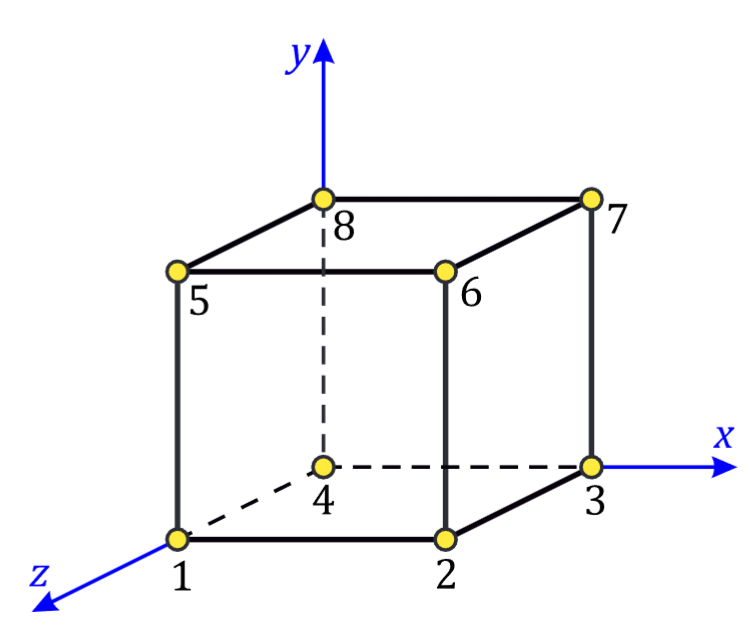
\includegraphics[scale=0.4]{figures/cube.png}
    \caption{Nodal layout of the brick element.}
    \label{fig:cube}
\end{figure}

We have a prescribed displacements on the upper nodes, defined by displacement vector as

\begin{equation}
    [\boldsymbol{U_1}] = [\boldsymbol{U_2}] = [\boldsymbol{U_3}] = [\boldsymbol{U_4}] = \begin{bmatrix} 0 & 0 & 0 \end{bmatrix}^T,
\end{equation}

\begin{equation}
    [\boldsymbol{U_5}] = [\boldsymbol{U_6}] = [\boldsymbol{U_7}] = [\boldsymbol{U_8}] = \begin{bmatrix} u_x & u_y & 0 \end{bmatrix}^T,
\end{equation}\\

where the time evolution of $u_x$ and $u_y$ and their time derivatives are shown on Figure \ref{fig:displacements}.

\begin{figure}[h]
    \centering
    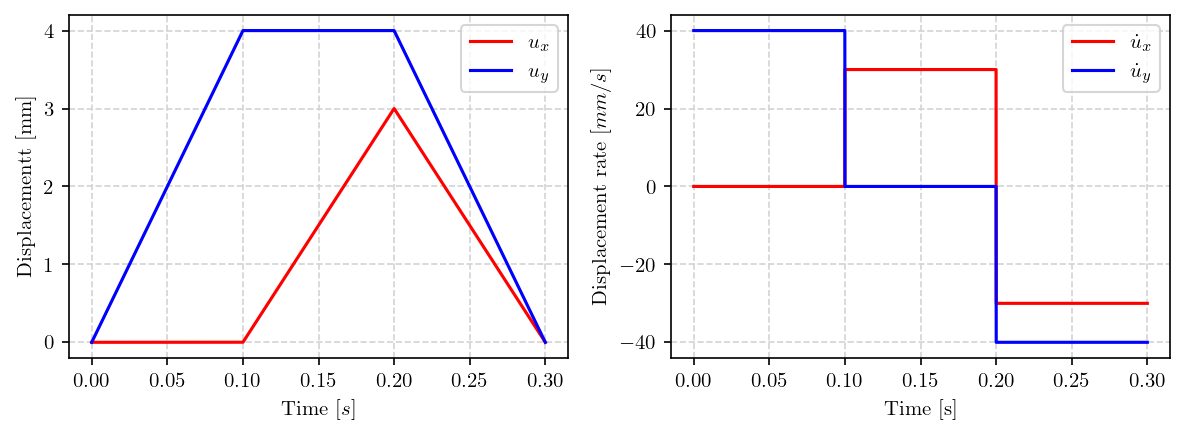
\includegraphics[width=0.8\textwidth]{figures/loading.png}
    \caption{The parameters of the loading}
    \label{fig:displacements}
\end{figure}

From the displacement vectors we can determine the deformations gradient regarding to that motion.

\begin{equation}
    [F] = 
        \begin{bmatrix}
            1 & u_x/L & 0 \\
            0 & 1+u_y/L & 0 \\
            0 & 0 & 1 \\
        \end{bmatrix}.
\end{equation}

\newpage

For the further calculations we will need the velocity gradiend, which can be calculated from the deformation gradient as

\begin{equation}
    [\boldsymbol{l}] = [\dot{\boldsymbol{F}}\boldsymbol{F}^{-1}] = 
        \begin{bmatrix}
            0 & \dot{u_x} & 0 \\
            0 & \dot{u_y} & 0 \\
            0 & 0 & 0 \\
        \end{bmatrix}
        \begin{bmatrix}
            1 & -\dfrac{u_x}{1 + u_y} & 0 \\
            0 & \dfrac{1}{1 + u_y} & 0 \\
            0 & 0 & 1 \\
        \end{bmatrix}
        =
        \dfrac{1}{1 + u_y}
        \begin{bmatrix}
            0 & \dot{u_x} & 0 \\
            0 & \dot{u_y} & 0 \\
            0 & 0 & 0 \\
    \end{bmatrix}
\end{equation}

The rate of deformation ($\boldsymbol{d}$) is the symmetric and the spin tensor ($\boldsymbol{w}$) is the skew symmetric part of the velocity gradient:

\begin{equation}
    \boldsymbol{d} = \frac{1}{2}(\boldsymbol{l}+\boldsymbol{l}^T) \quad\&\quad \boldsymbol{w} = \frac{1}{2}(\boldsymbol{l}-\boldsymbol{l}^T).
\end{equation}  

\section*{Material behaviour}

This element has an elastic-plastic behaviour. We have finite deformations, therefore we need to use hypoelastic-plastic modelling approach, which is based on the additive decomposition of the rate of deformation tensor into elastic and plastic part

\begin{equation}
    \boldsymbol{d} = \boldsymbol{d}^e + \boldsymbol{d}^p.
\end{equation}  

Following the ABAQUS formulation, the elastic behaviour can be defined by the Hooke's law as follows

\begin{equation}
    \overset{\circ}{\boldsymbol{\sigma}}  = \frac{E}{1+\nu}\left(\boldsymbol{d}^e+\frac{\nu}{1-2\nu}(\text{tr}\boldsymbol{d}^e)\boldsymbol{I}\right) := \mathbb{D} : \boldsymbol{d}^e,
\end{equation}

where the $\overset{\circ}{\boldsymbol{\sigma}}$ denotes the Jaumann rate of the Cauchy stress tensor. The discrete form of the Hooke's law in the rotated coordinate system looks like 

\begin{equation}
    \tilde{\boldsymbol{\sigma}}_{n+1}  = \tilde{\boldsymbol{\sigma}}_{n} + 
    \mathbb{D} \Delta\tilde{\boldsymbol{\varepsilon}}^e
\end{equation}

To be able to rotate the quantities back and forth, we need to determine the $\boldsymbol{Q}$ rotation tensor in each step, which can be calculated from the $\boldsymbol{w}$ spin tensor as

\begin{equation}
    \dot{\boldsymbol{Q}} = \boldsymbol{w}\boldsymbol{Q},
\end{equation}

where we can conclude that we will need time integration to determine the values. We will use the Hughes-Winget algorithm as it is required, which is defined as 

\begin{equation}
    \boldsymbol{Q}_{n+1} = \left(\boldsymbol{I} - \frac{1}{2} \boldsymbol{w}_{n+1/2} \Delta t \right)^{-1} 
\left(\boldsymbol{I} + \frac{1}{2} \boldsymbol{w}_{n+1/2} \Delta t \right) 
\boldsymbol{Q}_n.
\end{equation}

The values of the elastic material parameters are the followings

\begin{equation}
    E = 200 \;\text{GPa} \quad\&\quad \nu = 0.3
\end{equation}

Furthermore the characteristic of the Yield stress is defined by the following Swift model:

\begin{equation}
    Y(\lambda) = a(\varepsilon_0+\lambda)^n\quad \text{,where} \quad a=400\;\text{MPa,} \quad \varepsilon_0=0.05, \quad n=0.25.
\end{equation}

\newpage

\section*{Solution}

My implementation of the radial-retirn algorithm for this hypoelastic-plastic model in Python language is the following:

\lstset{style=python}
\begin{lstlisting}
Q = np.tile(I, (N, 1, 1))
sig_tilde = np.tile(O, (N, 1, 1))
sig = np.tile(O, (N, 1, 1))
Y = np.ones(N) * Y_F(0)
_lambda = np.zeros(N)

for n in range(N-1):
    dt = t[n+1] - t[n]
    w_mid = (w[n+1] + w[n])/2
    d_mid = (d[n+1] + d[n])/2

    # Hughes-Winget
    Q[n+1] = inv(I - 1/2*w_mid*dt) @ (I + 1/2*w_mid*dt) @ Q[n]
    Q_mid = Q[n+1] 

    deps_tilde = Q_mid.T @ d_mid* dt @ Q_mid

    # Step 3: trial stress
    sig_trial_tilde = sig_tilde[n] + D(deps_tilde)
    s_trial_tilde = dev(sig_trial_tilde)

    # Step 4: trial yield function
    F_trial = (3/2)**(1/2) * norm(s_trial_tilde) - Y[n]

    if F_trial <= 0:
        # Step 6: Elastic increment
        sig_tilde[n+1] = sig_trial_tilde
        Y[n+1] = Y[n]
        _lambda[n+1] = _lambda[n]
    else:
        # Step 7: Accumulated plastic strain increment
        def eq(d_lambda):
            ret  = (3/2)**(1/2) * norm(s_trial_tilde)
            ret -= 3*G*d_lambda
            ret -= Y_F(_lambda[n]+d_lambda)
            return ret
        d_lambda = (root(eq,1e-8).x)[0]
        
        # Step 8: Plastic strain increment and yield stress update
        deps_p_tilde = (3/2)**(1/2) * d_lambda * s_trial_tilde / norm(s_trial_tilde)
        _lambda[n+1] = _lambda[n] + d_lambda
        Y[n+1] = Y_F(_lambda[n+1])
        
        # Step 9: Update the rotated stress
        sig_tilde[n+1] = sig_trial_tilde - D(deps_p_tilde)
    
    # Step 10: Compute the stress tensor
    sig[n+1] = Q[n+1] @ sig_tilde[n+1] @ Q[n+1].T
\end{lstlisting}

\newpage

\subsection*{5 increments per step}

The values of the plotted quantities are also attached as a CSV file.

\begin{figure}[h]
    \centering
    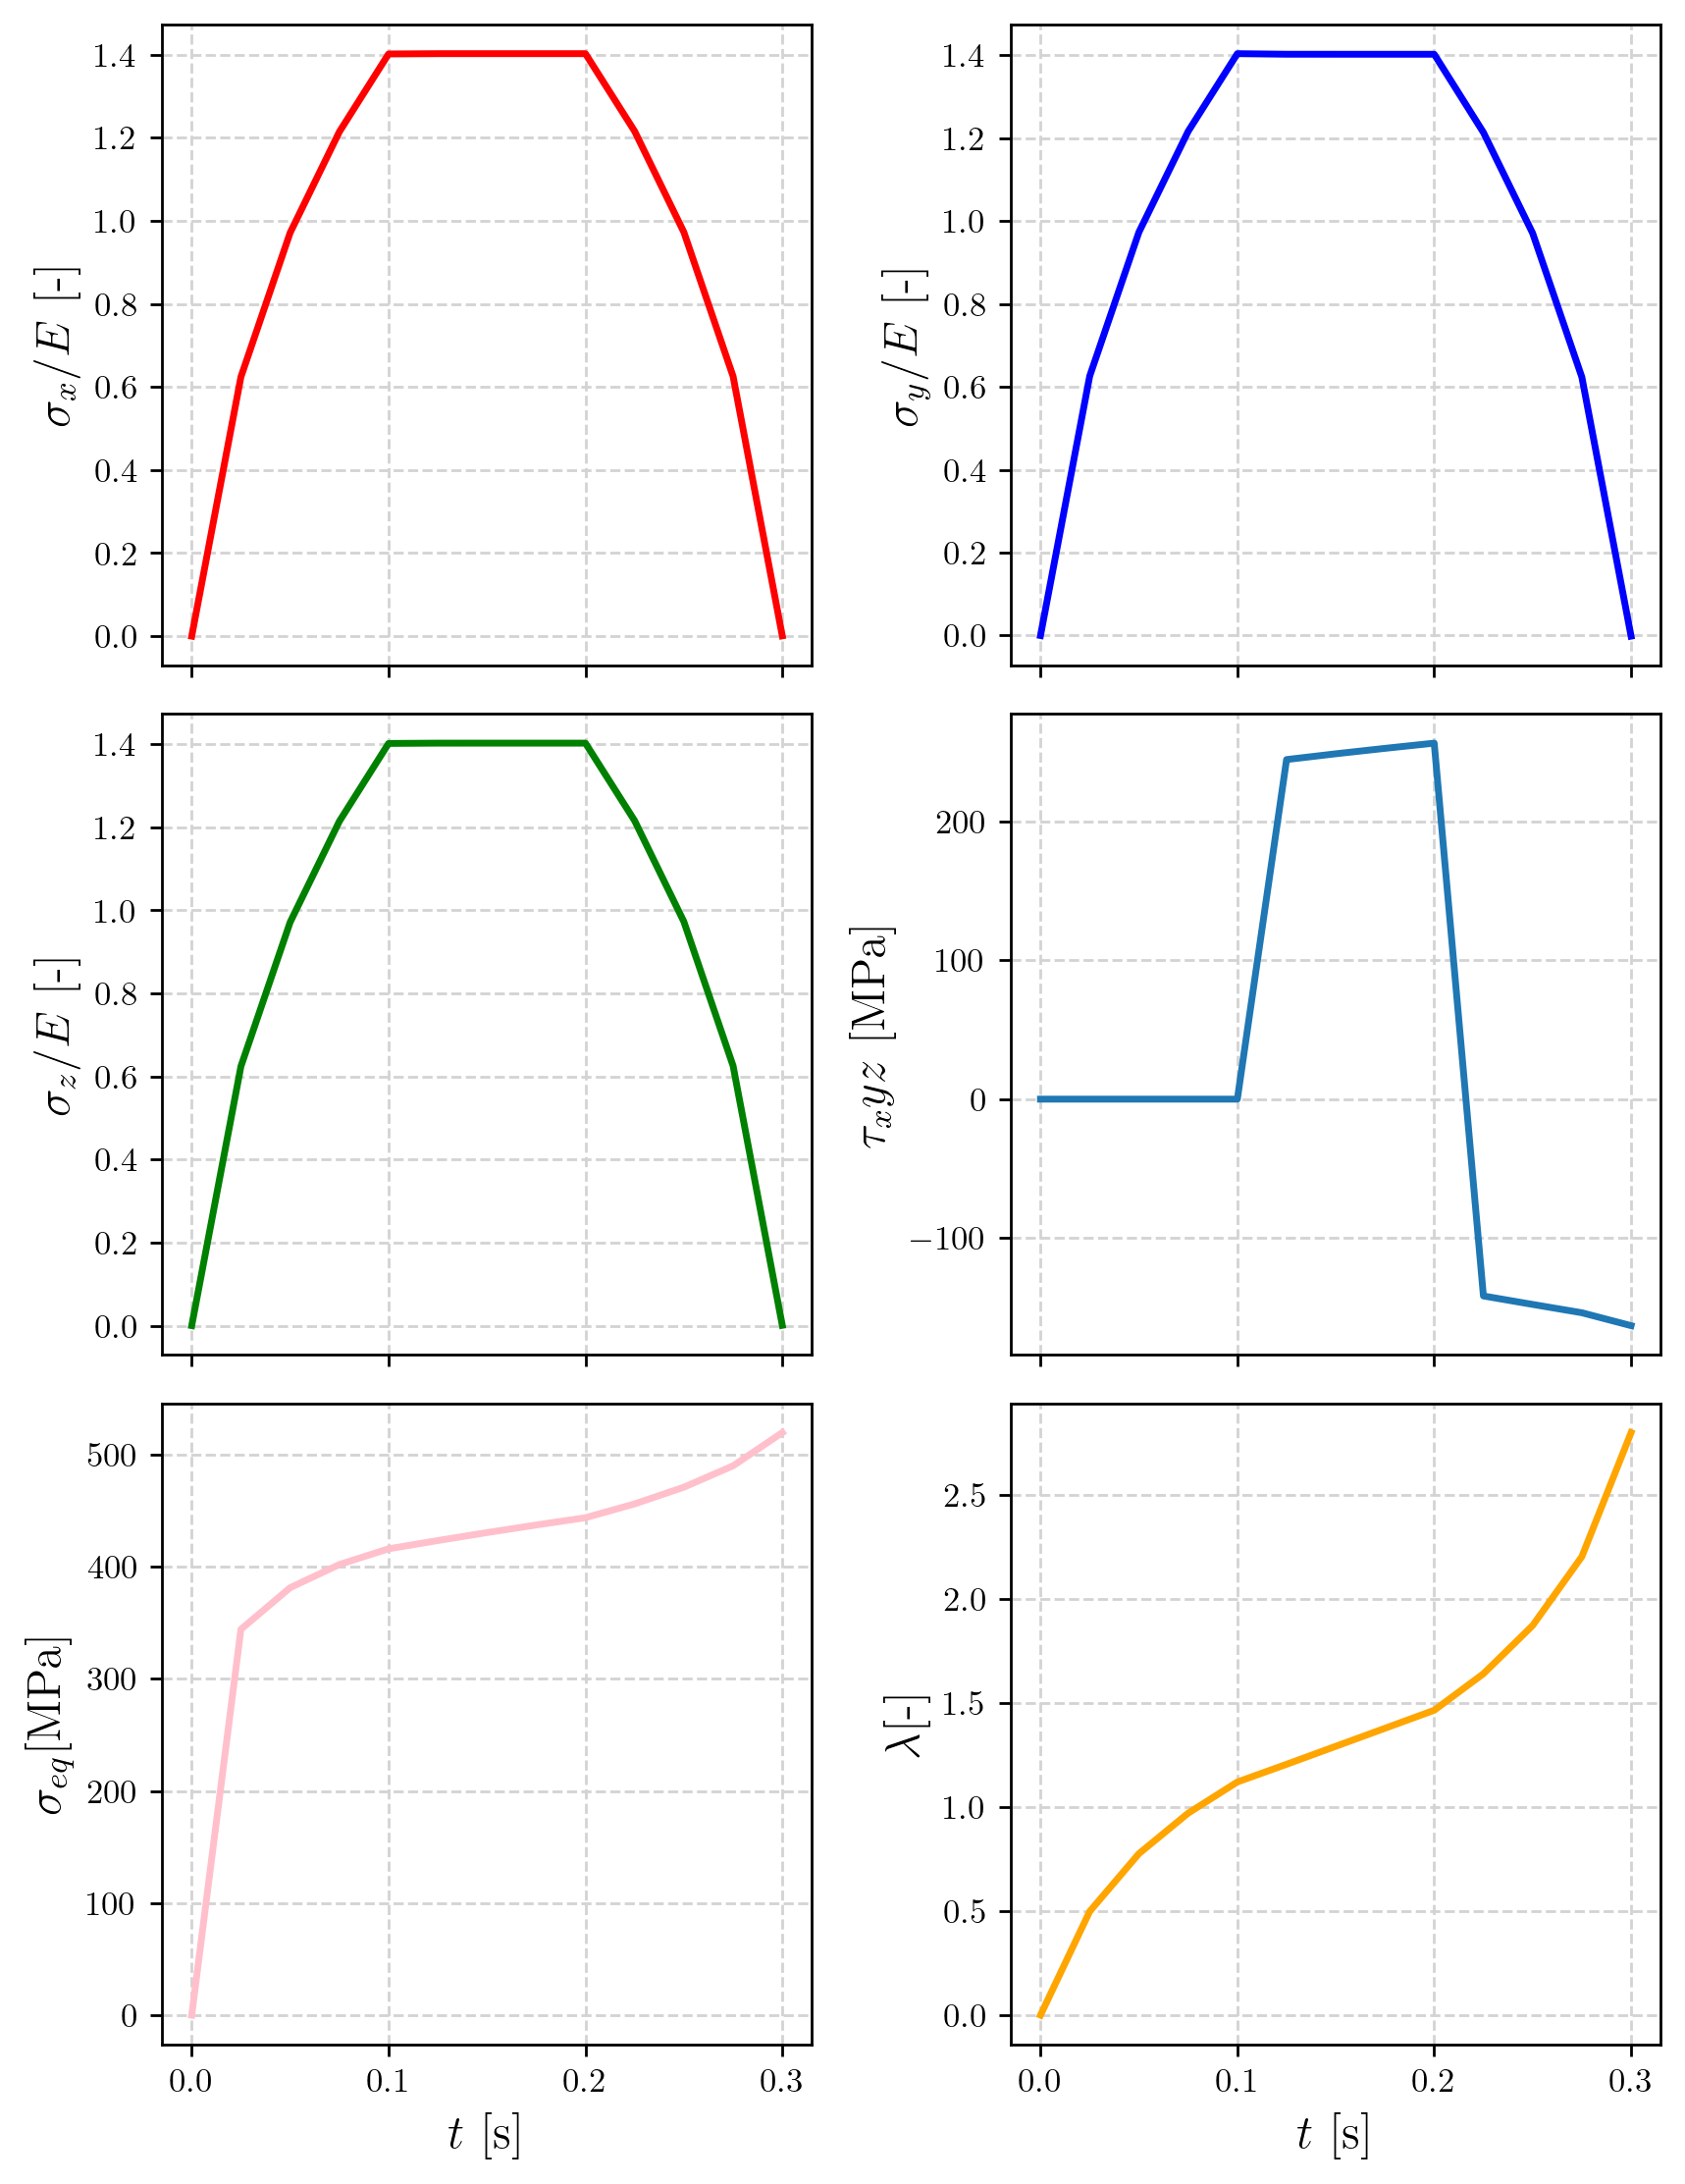
\includegraphics[width=0.8\textwidth]{figures/sol_5incr.png}
    \caption{The solution of the problem, by applying 5 increments in each step.}
    \label{fig:sol_5incr}
\end{figure}

\newpage

\subsection*{1000 increments per step}

The values of the plotted quantities are also attached as a CSV file.

\begin{figure}[h]
    \centering
    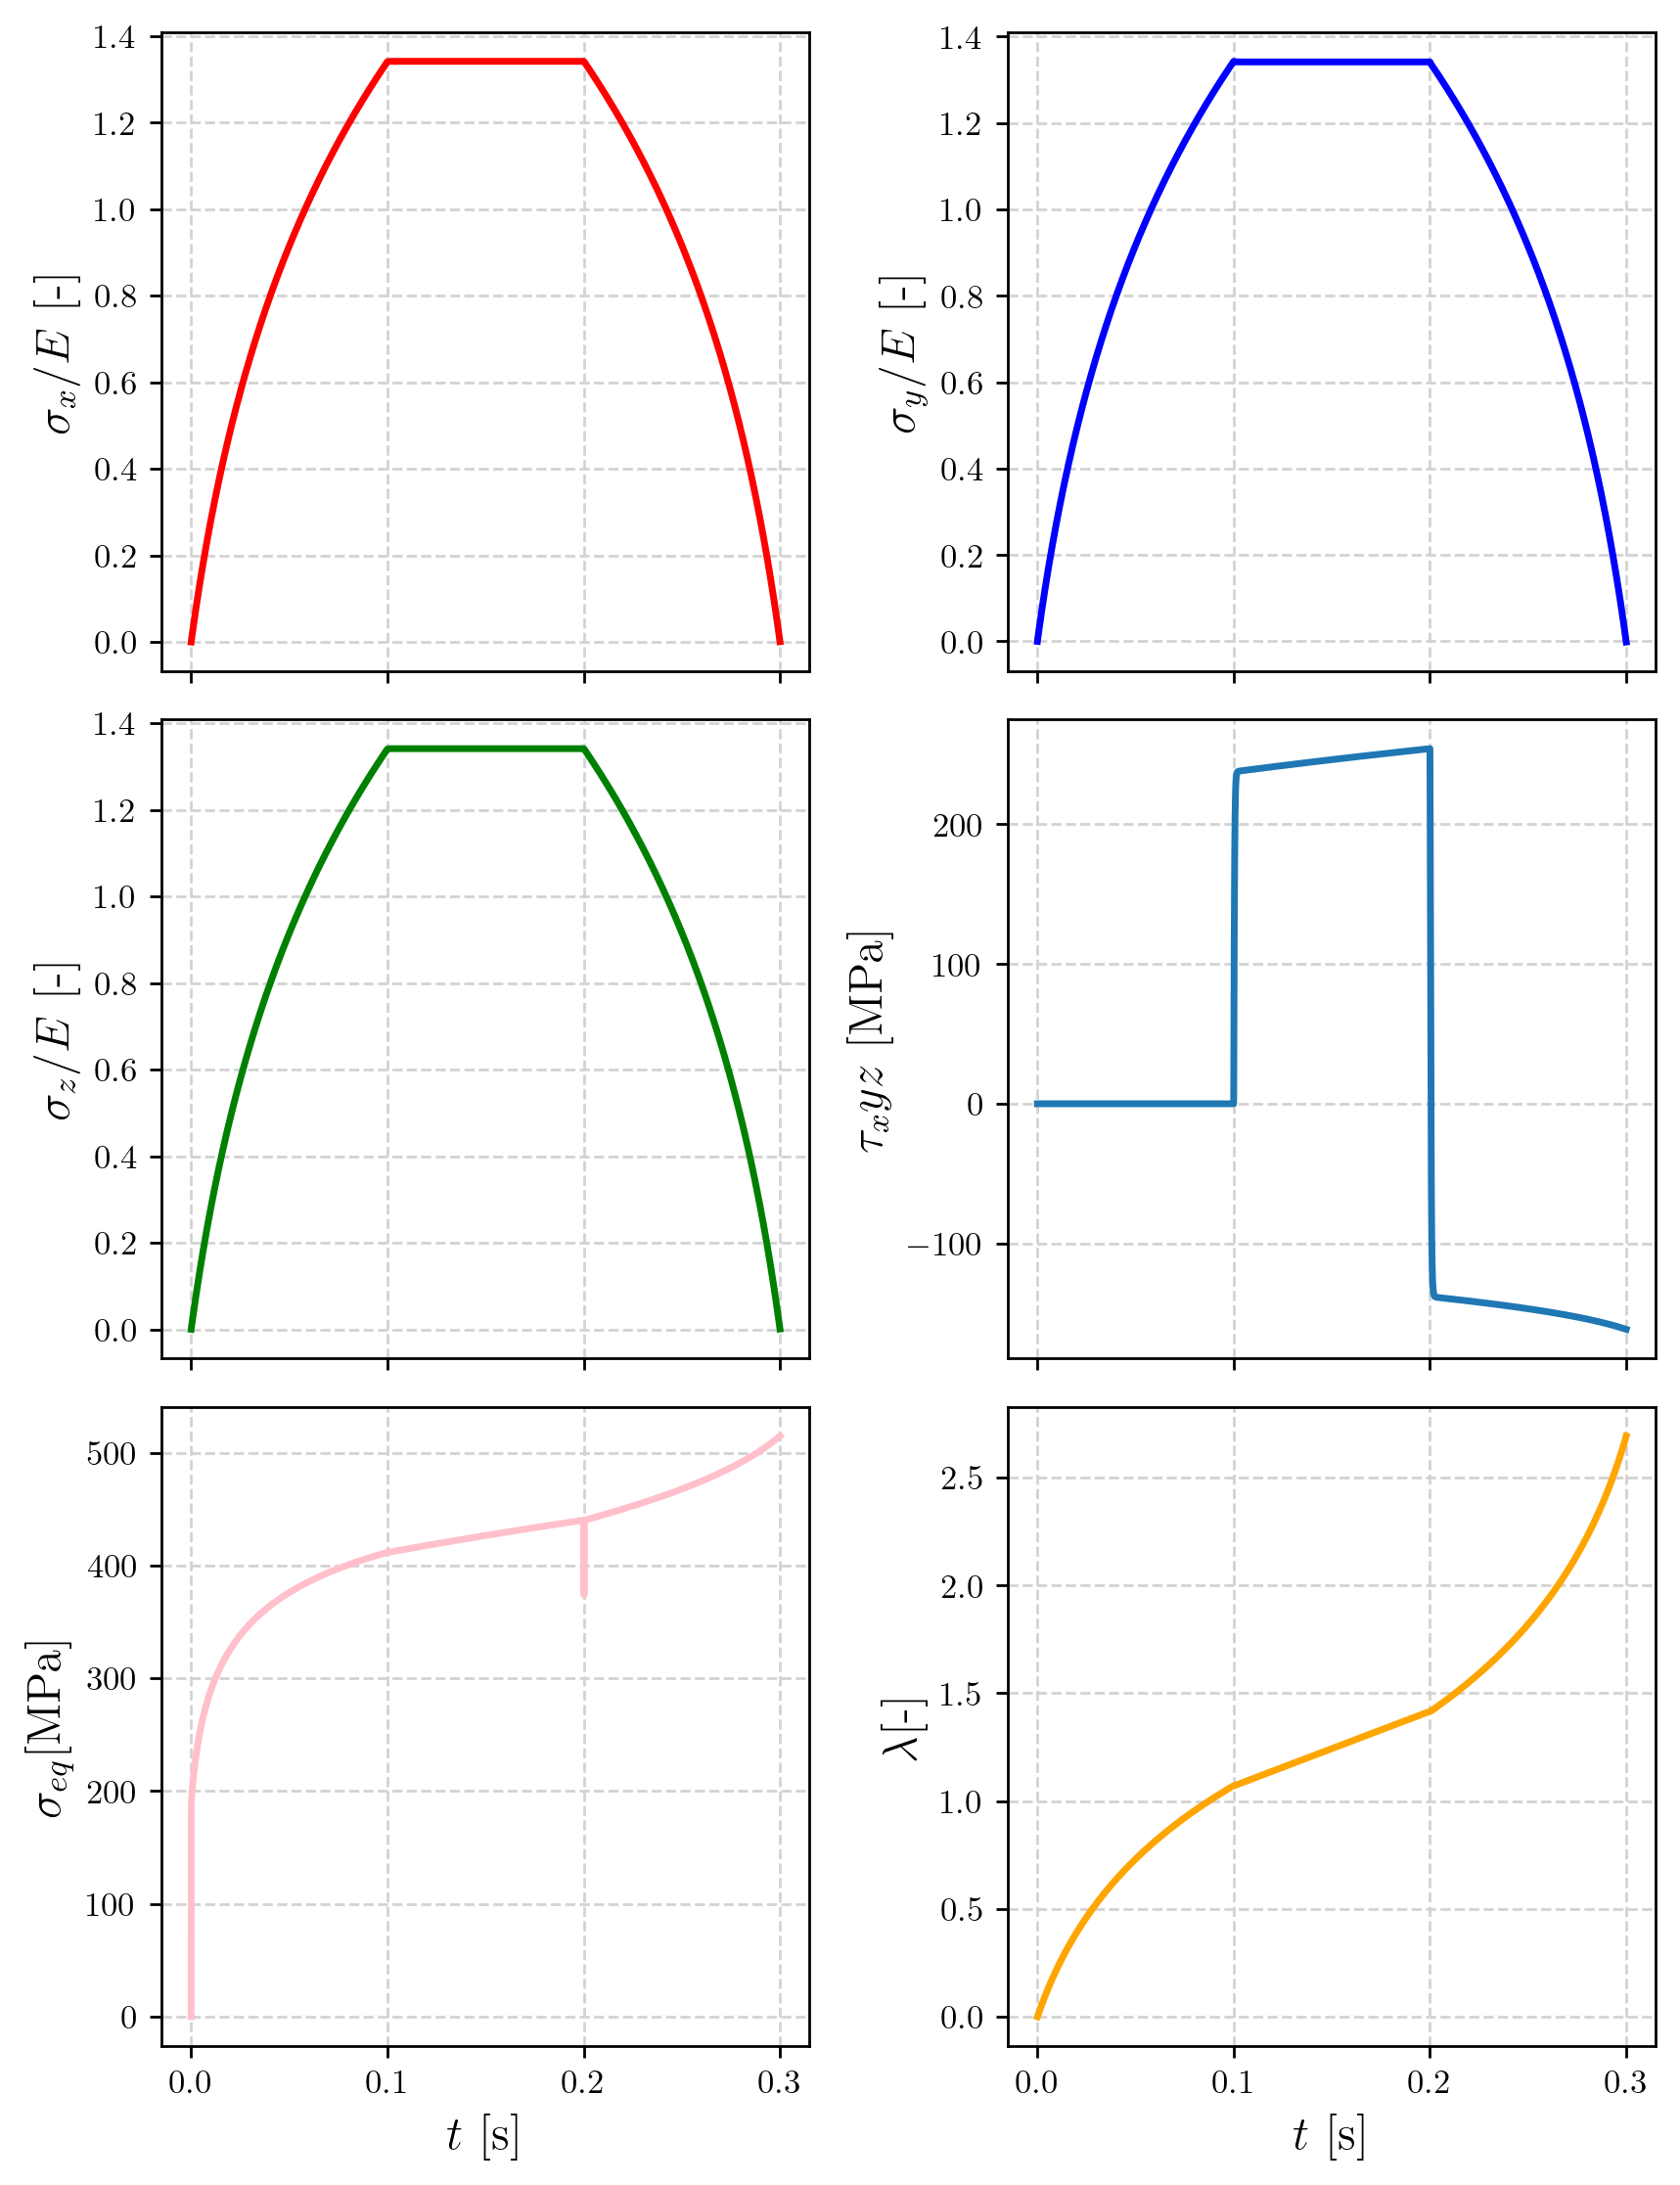
\includegraphics[width=0.8\textwidth]{figures/sol_1000incr.png}
    \caption{The solution of the problem, by applying 1000 increments in each step.}
    \label{fig:sol_1000incr}
\end{figure}

\newpage

\section*{References}

You can find the detailed code on \href{https://github.com/zsoca000/Finite-elastic-deformations-HW2/blob/main/calculations.ipynb}{\textcolor{blue}{\underline{GitHub}}}.

\end{document}